%% THINGS TO DO %%
% - EDIT ALL TABLES: SIZES, BOLD, ETC.. %
% - HOW TO MAKE A BOLD ROW %
% - ADD IN SOLDERED BATTMON BOARD %
% - ADD IN SOLDERED LED BOARD %

\subsection{Electronics}

%% SYSTEM OVERVIEW %%
\subsubsection{System Overview}
The electronics architecture has been improved from the design proposed by the WMR 2014/15 team.\par

\begin{figure}[ht]
\centering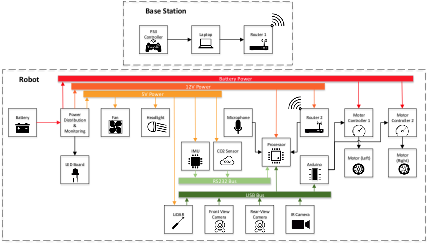
\includegraphics[width=0.8\linewidth]
{Images/ElectronicsFigures/ElectronicsBlockDiagram.png}
\caption{Electronics Systems Diagram}
\label{fig:eleoverview}
\end{figure}

The key differences include the addition of a second router at the base station. This approach has been implemented to overcome the ‘connectivity issues’ that many past WMR teams have experienced at the competition. The new router has superior performance over a laptops Wi-Fi card and so will improve the connectivity between the robot and the base station.\par

A second key difference is the removal of the bulky 8-to-1 USB splitter. This device limited the speed that the USB peripherals can run at, bottle-necking 8 data streams into 1, due to the maximum capable speed on USB 2.0. To ensure good quality video streams, it is proposed the RS232 ports of the robot's computer are utilised. Both the CO2 sensor and Inertial Measurement Unit (IMU) have compatible RS232 outputs.\par

It was discovered that a single threaded microcontroller could not reliably support the control of the motors whilst pseudo-simultaneously monitoring sub-systems. Therefore, a dedicated microcontroller is proposed for each motor, with the option to change this to a multi-threaded device in the future should additional sensors be required.\par

The final distinct difference regards the rationalisation of the power distribution and battery monitoring board from two separate entities into one, plus the addition of a dedicated LED board.\par

%% PROCESSOR %%
\subsubsection{Processor}
A quintessential component within the robot is the processor board. This board runs the Ubuntu OS and the ROS master software, so is responsible for managing each of the subsystems simultaneously, whilst maintain a live feed of information to the base station laptop. A range of processor boards were considered and the results against the requirement criteria are given in Table \ref{tab:procomp}.\par

% MAKE SOME ROWS/COLUMNS BOLD? %
\begin{table}[ht]
\resizebox{\linewidth}{!}{
\begin{tabular}{>{\bfseries}c c s s c s s s c }
\toprule
\multicolumn{1}{c}{}& & \multicolumn{2}{c}{Power Supply} & \multicolumn{3}{c}{Processing} & \multicolumn{2}{c}{I/O Capability} \\
\cline{3-9}
 & Dimensions& Voltage & Power & & Speed & DDR3 & & \\
Processor Board & (mm) & (V) & (W) & Chipset & (GHz) & (GB) & USB & Other\\
\hline
Axiotex PICO831 & 100 x 72 & 5 & 15 & Intel Atom N2800 & 1.86 & 4 & 4 & 2x RS232  \\ 
Intel NUC5i5MYBE & 115 x 111 & 19 & 65 & Intel Core i5 & 2,3 & 16 & 6 & -  \\ 
Axiotex PICO842 & 100 x 72 & 12 & 10,8 & Intel Celeron J1900 & 2,42 & 8 & 4 & 2x RS232 \\ 
\hline
\end{tabular}
}
\caption{Processor Comparison}
\label{tab:procomp}
\end{table}
%[REF1 - 3]

Last year's WMR team chose the PICO831 as the robot computer shown above. This board utilises an Intel Atom N2800 chipset released in 2011 [RFE4] and can only support 4GB of DDR3 RAM capability. However, Cyclone requires a greater amount of RAM to support multiple, real-time camera feeds, so alternative options were considered.\par

The Intel NUC board was a good choice as it outperforms the previous board with its capability to support 16GB RAM. In addition, its processor runs 23\% faster and has an additional 2 USB ports compared to Orion, this comes to the detriment of power with this board drawing over 4 times as much power as the previous design. It was decided therefore that the more recent, PICO842 board utilising the Intel Celeron J1900 released later in 2013, was the best option [REF5]. This processor coupled with the AX93283 I/O expansion board [REF6], with Gigabit Ethernet capability provides a fast processing platform at low power consumption, and so therefore was selected as the ideal choice for our robot application.\par

%% MOTORS %%
\subsubsection{Motors}
The WMR project team of 2014/15 set to use Maxon EC-4pole 323217 motors coupled with the Maxon ESCON P/N 409510 controllers. It was discovered that these motors were not suitable for our robot, as discussed in greater detail in [JOE’S SECTIONS]. Therefore, a new set of motors (plus gear head) that were capable of providing a greater torque were required. A second requirement was that the new motors are compatible with the existing controllers already purchased. Table \ref{tab:motcomp} provides a summary of the results from the motor investigation.\par

% MAKE SOME ROWS/COLUMNS BOLD? %
\begin{table}[ht]
\centering
\resizebox{0.75\linewidth}{!}{
\begin{tabular}{>{\bfseries}c c c c c c c}
\hline
Option Number & Old & 1 & 2 & 3 & 4 & 5 \\ \hline
Motor & 323217 & 136203 & 136204 & 370356 & 305015 & 305015 \\ 
\hline
\hline
Efficiency  & 0.88 & 0.8 & 0.8 & 0.94 & 0.9 & 0.9 \\ \hline
Speed constant  & 907 & 579 & 445 & 102 & 346 & 346 \\ \hline
Speed/Torque constant  & 27.8 & 6.78 & 6.67 & 0.666 & 4.83 & 4.83 \\ \hline
Torque constant  & 0.0105 & 0.0165 & 0.0214 & 0.0934 & 0.0276 & 0.0276 \\ \hline
\  & \  & \  & \  & \  & \  & \  \\ \hline
Gear & 166945 & 203127 & 203127 & 223087 & 203127 & 326669 \\ 
\hline
\hline
Ratio & 122.8 & 126 & 126 & 26 & 126 & 123 \\ \hline
Efficiency & 0.7 & 0.72 & 0.72 & 0.83 & 0.72 & 0.7 \\ \hline
\  & \  & \  & \  & \  & \  & \  \\ \hline
Motor controller & 4094510 & 409510 & 409510 & 409510 & 409510 & 409510 \\ 
\hline
\hline
Efficiency & 0.98 & 0.98 & 0.98 & 0.98 & 0.98 & 0.98 \\ \hline
Voltage drop & 1 & 1 & 1 & 1 & 1 & 1 \\ \hline
\multicolumn{7}{c}{Results}  \\
\hline
\hline
No load (rpm) * & 77.938 & 45.341 & 34.847 & 52.431 & 30.482 & 30.358 \\ \hline
Incline (rpm)* & 74.06 & 44.419 & 33.941 & 51.992 & 29.825 & 29.685 \\ \hline
No load (A) & 0.899 & 0.596 & 0.46 & 0.377 & 0.317 & 0.334 \\ \hline
Incline (A)** & 10.278 & 6.817 & 5.256 & 4.309 & 3.623 & 3.817 \\ \hline
\end{tabular}
}
\caption{Motor Comparison}
\label{tab:motcomp}
\end{table}

* Speed at 18.5V, the theoretical minimum worse case scenario accounting for uneven cell discharge from the LiPo battery.\par
** Torque up an incline approximately 8Nm
[REF 1- 5 (motors)] [REF – 6-10 (Gear)] [REF 11 – Controller] JOE HAVE SAME REFERENCES?\par

The results show the theoretical speeds and current requirements for each of the motor/gear combinations. Mechanically the best motors are option 1, as they provide the most torque with option 5 providing the least torque. Conversely, from an electronics perspective, the power required to achieve those torques have almost the inverse relationship. Option 4 and 5 appear enticing due to their low power consumption, but this does come at a penalty on speed, which may be too slow for the robots operation.\par

Therefore, it was decided that to satisfy both mechanical and electronic requirements option 3 would be the motors of choice. The 94\% efficient DC 370356 motors coupled with the 83\% efficient 223087 gear head, are approximately 27\% more efficient than the old motors. This is important to help maximise the robot’s battery life.\par

%% MOTOR DRIVE PROCESSOR %%
\subsubsection{Motor Drive Processor}
The DC motors are managed via ESCON 50/50 P/N 409510 motor controllers. The motor velocity commands can be input by either an analogue or pulse-width-modulated (PWM) signal. Cyclone utilises the PWM functionality, as is boasts significant advantages particularly due to its insensitivity to noise. This trait is common across all digital signals, which has lead to their abundant usage in modern day electronics.\par

It was decided that the ATMega328 microcontroller on the Arduino Uno platform was suitable for this application. This cheap microcontroller is smaller and requires less power when compared to the Arduino Mega 2560 board; as proposed by the WMR 2014/15 team. In addition, an Arduino can be easily integrated with the ROS environment, plus software development is made easy with the intuitive Arduino IDE.\par

%% SENSOR ARRAY %%
\subsubsection{Sensor Array}
In order for the robot to compete at the RoboCup, it needs to be equipped with a range of sensors, and the greater the capability of the robot, the more points it will be awarded. It is for this reason that Cyclone’s architecture has been designed to handle a comprehensive range of sensors. Although the sensor arrays used in previous WMR builds are proven designs, a revision of these are required for Cyclone. The key reason for this is to take advantage of the latest cutting edge technology, whilst ensuring their compatibility with the ROS driven system within Cyclone. Table \ref{tab:sensarray} gives a summary of the sensors that will be used in Cyclone.\par

% MAKE SOME ROWS/COLUMNS BOLD? %
\begin{table}[ht]
\resizebox{\linewidth}{!}{
\begin{tabular}{c c c c c }
\hline
Sensor & \multicolumn{2}{c}{Part} & Own or Required & Interface  \\ \cline{2-3}
& Company & Part Number & & \\ \hline
LiDAR & Hokuyo & URG-04LX & Own & USB \\ \hline
IR Camera & Photon & 160 & Own & USB \\ \hline
Front-View Camera & - & - & Required & USB \\ \hline
Rear-View Camera & Microsoft & LifeCam HD-3000 & Own & USB \\ \hline
IMU & Xsens & MTi-28A53G35 & Own & RS232 \\ \hline
CO2 Sensor & DFR & SEN0159 & Own & RS232 \\ \hline
Microphone & - & - & Required & Microphone \\ \hline
Headlight & - & - & Required & - \\ \hline
\end{tabular}
}
\caption{Cyclones Sesnor Array}
\label{tab:sensarray}
\end{table}


%% BATTERY MONITOR BOARD - OVERVIEW %%
\subsubsection{Battery Monitor Board}
\paragraph{Overview}
The 2014/15 WMR team designed and manufactured a power distribution board. It was capable of providing regulated power at 12V or 5V to each robot subsystem. However, after a critical analysis of the board it was decided a redesign was needed for the following reasons:\par

\begin{enumerate}
\item When tested, the 12V regulator was not producing the required output. It would require major board modifications, which are not easy to do on buried PCB traces.
\item The 5V regulator was not appropriate for the design, due to over cautious estimations of its output power requirement. This meant it would operate at a much lower efficiency than expected. It would severely reduce the robots battery life and cause the regulator to get undesirably hot. 
\item The max current output from the 12V regulator was too small and it would not have been capable of powering the new processor board. 
\item There was no consideration for how battery monitoring and automatic shutdown of the robot could be implemented. Additionally, there was no consideration for how a master power switch and E-Stop button would be integrated. 
\item There were redundant current limiting fuses that would not have blown in the event of an over-current draw.
\item The design has neither an output to drive the motors or the raw battery voltage that may be required in the future design of an arm.
\end{enumerate}

%% BATTERY MONITORING - PRINCIPLE OPERATIONS %%
\paragraph{Principle Operations}
A new integrated battery distribution \& monitoring board was therefore designed, with the schematic given in [APPENDIX 1]. The robot utilises Lithium-Polymer (LiPo) batteries due to their compact size, large capacity and high discharge rate. These are volatile as they use dry electrolyte polymer sheets, which can burst or catch fire if mistreated [REF1]. So each of the batteries cells are monitored to ensure they stay within their safe operating conditions, whilst also ensuring their maximum power is drawn from them.\par

It is for this reason that an ATMega328 microcontroller is required on the board. It has 6x 10-bit ADC inputs, which are used to monitor each of the cells to an accuracy of 4.88mV. The microcontroller updates an LED array with the current battery voltage, in addition to sending messages back through ROS to display this level on the operators GUI. Not only this, but should the warnings be ignored, the microcontroller will automatically shut down the entire robot, to ensure the safety and longevity of the battery.\par

An additional safety feature this microcontroller handles is the monitoring of sub-systems ‘heartbeats’. The electronic systems output periodic pulses when operating correctly, which can be monitored. In the event of a software glitch, the ‘heartbeat’ is not received, and the operation of the robot is likely to be unknown and uncontrollable; this also causes the controller to shut down the robot, as a precaution. The battery status LED would begin to flash at an identifiable frequency, so that the reason for the shutdown is known.\par

Some additional hardware safety features have also been incorporated into the design. An emergency stop and master power on/off switch have been included like many previous successful WMR designs. These switches had to be selected carefully to ensure they fulfilled the power requirements of Cyclone.\par

%% BATTERY MONITORING - VOLTAGE REGULATORS %%
\paragraph{Voltage Regulators}
The design team from last year had to make conservative estimations on the power drawn from each device. These values accounted for the worse case scenario and in cases were poor estimations of the true power drawn. Table \ref{tab:pwrreq} gives the updated power requirements of each of the devices. Note that to improve the accuracy of the results, some components have been measured using the actually device connected to a bench power supply.\par

% MAKE SOME ROWS/COLUMNS BOLD? %
\begin{table}[ht]
\resizebox{\linewidth}{!}{
\begin{tabular}{c c c c}
\hline
Device & Voltage (V) & Max Current (A) & Safety Margin  (+20\%) (A) \\ 
\hline
\hline
Motor (x2) & Battery & 8.6 & 10.32 \\ \hline
Motor Controllers (x2) & Battery & 0.172 & 0.2064 \\ \hline
\multicolumn{3}{r}{Total} & 10.5264 \\ 
\hline
\hline
Processor & 12 & 0.9 & 1.08 \\ \hline
Arduino (Motors) & 12 & 0.1 & 0.12 \\ \hline
Front Camera & 12 & 0.5 & 0.6 \\ \hline
Rear-View Camera & 12 & 0.5 & 0.6 \\ \hline
IR Camera & 12 & 0.5 & 0.6 \\ \hline
\multicolumn{3}{r}{Total} & 4.2 \\ 
\hline
\hline
Router & 12 & 1 & 1.2 \\ \hline
LiDAR & 5 & 0.5 & 0.6 \\ \hline
IMU & 5 & 0.07 & 0.084 \\ \hline
CO2 Sensor & 5 & 0.2 & 0.24 \\ \hline
Headlight & 5 & 0.35 & 0.42 \\ \hline
Fan & 5 & 0.236 & 0.2832 \\ \hline
\multicolumn{3}{r}{Total} & 1.6272 \\ 
\hline
\hline
\end{tabular}
}
\caption{Cyclones Power Requirements}
\label{tab:pwrreq}
\end{table}
%  [REF – ALL DATASHEETS?] %

A change in processor board coupled with these conservative estimates meant, the 5V regulator was overestimated and the 12V regulator was underestimated. Table \ref{tab:pwrreq} shows that the 1.63A and 4.20A are required from the 5V and 12V regulators respectively. The GE EHHD024A0A41 could supply 24A and the TRACO TEL30-2412 could provide a 2.5A output [REF2,3]. Figure \ref{fig:old5vg} shows an extracts from the GE EHHD024A0A41 datasheet.\par

\begin{figure}[ht]
\centering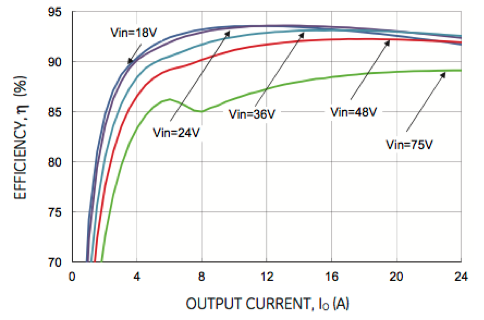
\includegraphics[width=0.8\linewidth]
{Images/ElectronicsFigures/RegulatorsGraph.png}
\caption{GE EHHD024A0A41 Efficiency against Output Current}
\label{fig:old5vg}
\end{figure}

This extract shows that at Cyclones expected current draw, this regulator would only be operating at around 70\% efficiency. So for these reasons a new set of regulators was considered. Table \ref{tab:regcomp} shows a comparison between the old and new components.\par

% MAKE SOME ROWS/COLUMNS BOLD? %
\begin{table}[ht]
\resizebox{\linewidth}{!}{
\begin{tabular}{c c c c c}
\hline
Part & Output Voltage (V) & Max Output Current (A) & Dimensions & Efficiency  \\ 
\hline
\hline
\multicolumn{5}{c}{WMR Power Distribution Board 2014/15} \\ \hline
TRACO TEL30-2412 & 12 & 2.5 & 2” x 1” & 0.91 \\ \hline
GE EHHD024A0A41 & 5 & 24 & 2.3” x 0.9” & \~70\% \\ \hline
\multicolumn{5}{c}{WMR Power Distribution Board 2015/16} \\ \hline
TRACO TEN60-2412N & 12 & 5 & 2” x 1” & 0.92 \\ \hline
TRACO TEN40-2411N & 5 & 8 & 2” x 1” & 0.91 \\ \hline
\end{tabular}
}
\caption{Regulators Comparison between Orion and Cyclone}
\label{tab:regcomp}
\end{table}
% [REF – 2,3,4,5] %


The TRACO TEN60-2412N and TRACO TEN40-2411N have been selected due to their high efficiency and small footprints. These rugged regulators satisfy the temperature requirements of the board with a wide operating range of \SI{-40}{\degree}C to \SI{+80}{\degree}C. Their maximum current outputs are greater than those calculated in Table \ref{tab:pwrreq}, but this is to allow for future expansion, with the inclusion of a robot arm.\par

\paragraph{Current Protection}
An over-current protection fuse has been incorporated into the design. The 25A Littelfuse was selected, such that if the current draw exceeded the expected maximum, allowing for a 20\% margin, then it would blow cutting the power to the robot.\par

\paragraph{Connectors}
This design requires many types of connectors, due to the number of mixed signal utilised in the design. All the connectors used within the robot were sourced from WMR sponsor, Harwin. Table \ref{tab:connectors} lists the selected connectors and identifies how they meet their associated requirements.\par

% MAKE SOME ROWS/COLUMNS BOLD? %
\begin{table}[ht]
\resizebox{\linewidth}{!}{
\begin{tabular}{c c c c c}
\hline
Purpose & Part Number & Gender & Quantity & Reason for Selection \\ \hline
Power & M80-5000000M2-02-331-00-000 & Male & 16 & Max current 20A per pin \\ \hline
Power & M80-4000000F1-02-325-00-000 & Female & 16 & Mating half \\ \hline
Heartbeat & M80-8810245 & Male & 2 & Friction Latches  \\ \hline
Heartbeat & M80-8990205 & Female & 2 & Mating half \\ \hline
LED Board & M80-8630842 & Male & 2 & Friction Latches \\ \hline
LED Board & M80-8890805 & Female & 2 & Mating half \\ \hline
Battery Mon & M80-8631042 & Male & 1 & Friction Latches \\ \hline
Battery Mon & M80-8891005 & Female & 1 & Mating half \\ \hline
USB Board & M20-9710645 & Male & 1 & Compatible pin pitch to USB board \\ \hline
\end{tabular}
}
\caption{Harwin Connectors Used on Cyclones Battery Monitoring \& Distribution Board}
\label{tab:connectors}
\end{table}
% [REF 1-9] %

Harwin’s MixTek range of connectors can support up to 20A of current through each pin so will suffice the power distribution operations. Conversely, It was decided that their L-Tek range was suitable for all the low power signals. All of the connectors listed contain either, a screw terminal lock in or a friction latch (12-14N of force). These were selected to ensure a reliable connection, even under the shock and vibration conditions the robot will be subject to at the competition.\par

\paragraph{Trace Sizings}
The track widths on the board needed to be sized to suffice the power requirements previously stated. The trace sizings calculated in Table \ref{tab:tracesize} are based on the worse case scenario using the IPC-2221 standard [REF1].\par

% MAKE SOME ROWS/COLUMNS BOLD? %
\begin{table}[ht]
\resizebox{\linewidth}{!}{
\begin{tabular}{ c c c c }
\hline
Trace & Max Current (with 20\% safety margin) (A) & Trace width Single-Sided (mm) & Trace width Double-Sided (mm) \\ \hline
Battery  & 13.78 & 7.35 & 3.68 \\ \hline
12V & 4.2 & 1.43 & 0.71 \\ \hline
5V & 1.63 & 0.39 & 0.19 \\ \hline
Signals & < 0.03 & Negligible & Not Necessary \\ \hline
\end{tabular}
}
\caption{Trace Sizings Required for each Power Line}
\label{tab:tracesize}
\end{table}

These sizings have been calculates on the standard trace thickness of 1$oz.ft^-2$ ($\approx$\SI{35}{\micro\meter}), allowing for a \SI{20}{\degree}C  rise of an external track when conducting; with an assumption of \SI{25}{\degree}C ambient temperature [REF2]. The board design utilises double sides traces to minimise trace width, with the plated through holes to electrically connect the two. It was decided that there were enough through-hole connections, such that resistance between the traces on each layer was negligible, so no additional ‘shorting‘ vias were required.\par

In addition, traces have been made as short as possible in order to reduce their resistance. A high parasitic resistance would lead to a voltage drop along the trace; this would introduce issues like a floating ground. Not to mention the power that will be lost, which is scarce within the robot. Traditionally, a multi-layer board is used to minimise these effects, but the additional cost and complexity is not required for this build.\par

\paragraph{Board Dimensions}
These considerations to minimise the amount of board real-estate were required to create a compact board that suffice the required mechanical dimensions. The central section of the robot is \SI{212 x 322 x 122}{\milli\meter}, so the board was sized to \SI{120 x 120}{\milli\meter}. Therefore, the board can be rearranged in many orientations, so that future teams could alter the arrangements if required. The Ultiboard layout is given in [FIGURE BELOW].\par

\begin{figure}[ht]
  \centering
  \begin{minipage}[b]{0.45\textwidth}
    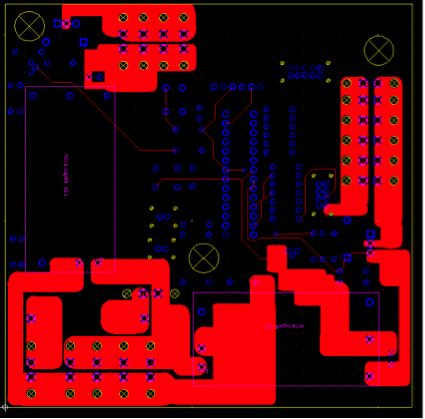
\includegraphics[width=\textwidth]{Images/ElectronicsFigures/BattMonBottom.png}
    \caption{Board Bottom-Side}
  \end{minipage}
  \hfill
  \begin{minipage}[b]{0.45\textwidth}
    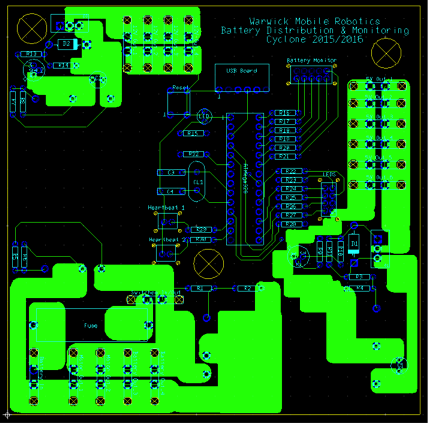
\includegraphics[width=\textwidth]{Images/ElectronicsFigures/BattMonTop.png}
    \caption{Board Top-Side}
  \end{minipage}
\end{figure}


\paragraph{Wire Sizings}
The wires carrying the current to and from the board also need to adhere to these power requirements. Table \ref{tab:wiresize} shows the wires thickness, in American Wire Gauge (AWG), selected from each part of the board [REF3].\par

% MAKE SOME ROWS/COLUMNS BOLD? %
\begin{table}[ht]
\resizebox{\linewidth}{!}{
\begin{tabular}{ c c c c }
\hline
Trace & Max Current (with 20\% safety margin) (A) & Wire Thickness (AWG) & Current Carrying Capability (A) \\ \hline
Battery  & 13.78 & 12 & 34 \\ \hline
12V & 4.2 & 14 & 24 \\ \hline
5V & 1.63 & 14 & 24 \\ \hline
Signals & < 0.03 & 22 & 5 \\ \hline
\end{tabular}
}
\caption{Wire Sizings Required for each Power Line}
\label{tab:wiresize}
\end{table}

\paragraph{Usability \& Testability}
A lot of thought went into the design to ensure maximum testability, plus the ability to modify the board if needed. In places, extra ‘dummy’ components where incorporated into the design with their pads laid out. However, the intention was to not fit these components, but have the ability to, should they be required during testing.\par

All components where selected to be through hole. This allowed ease of soldering and debugging of the board during testing. In addition, de-coupling capacitors where added to the outputs of the regulators. There purpose is to reduce the voltage ripple on their output, such that a smooth constant output is delivered to the remaining circuitry.\par

\paragraph{Component Placing}
Care was taken when placing the components in order to separate the high power ‘noisey’ circuitry, from the sensitive digital micro-controller circuits. In the designs layout, it was thought the regulators were placed on the backside of the board. The intention was these would be fixed to the robot casings, to aid with heat dissipation, whilst the connectors on the other side would still easily accessible to the rest of the sub-systems. However, there was a misinterpretation with the software and the regulators where not placed on the bottom of the board as expected.\par

\paragraph{Final Design}
The design was sent for manufacture at Euro circuits. They were selected as they could provide plated through holes, on a short-lead time, for at a reasonable price. The returned blank PCB was then populated with components, with the soldering done ‘in-house’ by hand, as shown in [FIGURE BELOW].\par

%% ADD SOLDERED PCB IMAGE - ON PHONE, CHNAGE REF ABOVE %%
% \begin{figure}[ht]
% \centering\includegraphics[width=0.8\linewidth]
% {Images/ElectronicsFigures/???.png}
% \caption{Battery Monitoring \& Distribution Board}
% \label{fig:finalboard}
% \end{figure}

\subsubsection{LED Board}
A second board was manufactured in the School of Engineering. This board consists of 6-power status LEDs and a robot status LED. This single sided board was design so that the LEDs can be placed externally from the previous board and can be made visible through the robot. All the routing is on a single-side of the board, however, the connector is orientation on the bottom side. This is so it can be connected on the inside of the robot, with the LEDs facing out of the robot. The 4 mounting holes allow the board to be fixed, with spacers to the robot using M3 screws.\par

%% ADD SOLDERED PCB IMAGE - ON PHONE, C %%
% \begin{figure}[ht]
% \centering\includegraphics[width=0.8\linewidth]
% {Images/ElectronicsFigures/???.png}
% \caption{LED Board}
% \label{fig:LEDboard}
% \end{figure}

